% !TEX root = ../main.tex

\section{Attack analysis}
Usually, \textit{transferFrom} function will be called after \textit{approve} method. The attack could happen in case of race condition\footnote{Execution of two transactions at the same time with undesirable situation or priority.}, that allows a spender to transfer more tokens than the owner ever wanted. This is possible since the \textit{approve} method overrides current allowance regardless of whether spender already transferred any tokens or not. Moreover, transferred tokens are not trackable and only \textit{Transfer}\footnote{Transfer(address indexed \_from, address indexed \_to, uint256 \_value)} event will be logged (which is not sufficient in case of transferring tokens to a third parity). Here could be a possible attack scenario:
\begin{enumerate}
	\item Alice allows Bob to transfer N tokens by calling \textit{approve(\_Bob, N)}.
	\item After a while, Alice decides to change Bob's approval from N to M by executing \textit{approve(\_Bob, M)}.
	\item Bob notices Alice’s second transaction before it was mined and quickly sends another transaction that runs \textit{transferFrom(\_Alice, \_Bob, N)}. This will transfer N Alice’s tokens to Bob.
	\item Bob’s transaction will be executed before Alice’s transaction (because of higher transaction fee, miner’s policy or other prioritization techniques) and Bob front-runs Alice’s transaction.
	\item Alice’s transaction will be executed after Bob’s and allows Bob to transfer more M tokens.
	\item Bob successfully transferred N Alice’s tokens and gains ability of transferring another M tokens.
	\item Before Alice notices that something went wrong, Bob calls \textit{transferFrom} method again and transfers M Alice’s tokens by executing \textit{transferFrom(\_Alice, \_Bob, M)}.\newline
\end{enumerate}

As its details are shown in the figure below, Alice attempted to change Bob’s allowance from N to M, but she made it possible for Bob to transfer N+M of her tokens at most, while Alice never wanted to allow so many transfers to be occurred by Bob:
\begin{figure}[H]
	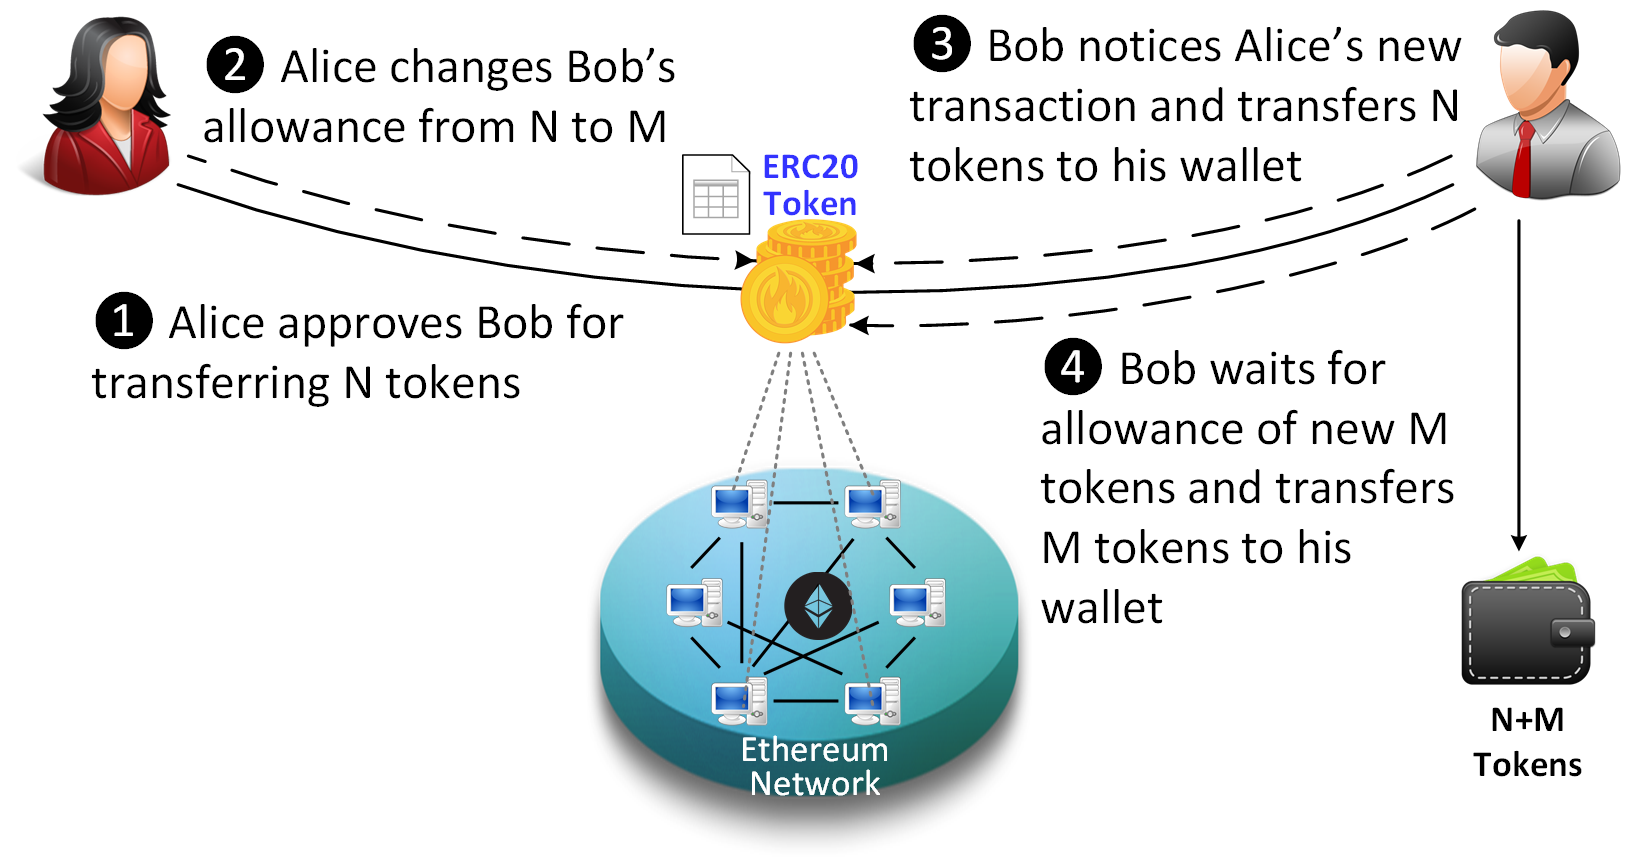
\includegraphics[width=1.0\linewidth]{figures/multiple_withdrawal_02.png}
	\caption{Possible multiple withdrawal attack in ERC20 tokens.}
\end{figure}
It should be noted that the assumption here is to prevent Bob from withdrawing Alice’s tokens multiple times. If he could withdraw N tokens after the initial Alice’s approval, this would be considered as legitimate transfer since Alice has already approved it. In other words, it is Alice’s responsibility to make sure before approving anything to Bob. In short, we are looking for a solution to prevent multiple withdrawal (N+M) by Bob presuming that Alice has more than N+M tokens in her wallet.